\documentclass[a4paper,11pt,final]{report}

\usepackage[utf8]{inputenc}
\usepackage[english]{babel}
\usepackage[T1]{fontenc}
\usepackage{longtable}
\usepackage{graphicx}
\usepackage{geometry}

\geometry{top=2cm,bottom=2cm,left=2cm,right=2cm}

\title{Lab 3 - TCP}
\author{Romain de Laage (romde686) \& Gyumin Park (gyupa395)\\Group A}
\date{\today}

\begin{document}
\maketitle

\chapter{TCP Basics}

\begin{enumerate}
\def\labelenumi{\arabic{enumi}.}
\item
  The first packet is number 4 (containing the POST verb and the HTTP
  headers), the last one is 199 (all the data is transmitted).
\item
  IP address of the client is 192.168.1.102 (in the IP headers) and TCP
  port number of the client is 1161 (in the TCP headers).
\item
  IP address of the server is 128.119.245.12 and TCP port number of the
  server is 80.
\item
  The SYN packet sequence number is 232129012. In the flags part of the
  TCP headers, the SYN flag is set to one.\\
  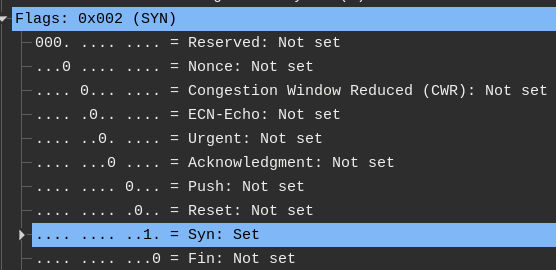
\includegraphics[width=0.7\linewidth]{upload_79bade8fe3ddf5c050bf59195e0e77e9.png}
\item
  The sequence number of the SYNACK packet is 883061785, the
  acknowledgment number is 232129013 (previous sequence number from the
  SYN packet plus 1). In the flags part of the TCP headers, the SYN flag
  and the ACK flag are set to one.\\
  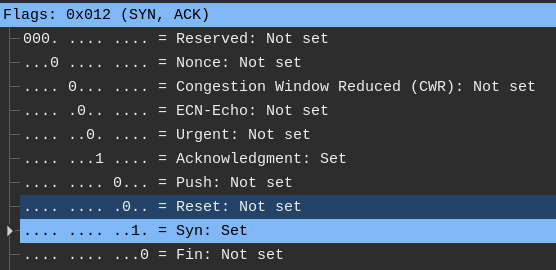
\includegraphics[width=0.7\linewidth]{upload_916fffa2f848e879e7481d83eff1193a.png}
\item
  The sequence number of the TCP segment containing the HTTP POST
  command is 232129013. This is the first packet for the POST request.
\item
  \(Estimated RTT = (1- \alpha) * Estimated RTT + \alpha * Sample RTT\)
\end{enumerate}

\begin{tabular}{|c|c|c|c|c|}
	\hline
Sequence number & Sending time (in seconds) & Ack time & Calculated RTT & Estimated RTT \\ \hline
232129013 & 1093095860.596858000 & 1093095860.624318000 & 0.02746 &
0.02746 \\ \hline
232129578 & 1093095860.612118000 & 1093095860.647675000 & 0.035557 &
0.028472125 \\ \hline
232131038 & 1093095860.624407000 & 1093095860.694466000 & 0.070059 &
0.033670484 \\ \hline
232132498 & 1093095860.625071000 & 1093095860.739499000 & 0.114428 &
0.043765174 \\ \hline
232133958 & 1093095860.647786000 & 1093095860.787680000 & 0.139894 &
0.055781277 \\ \hline
232135418 & 1093095860.648538000 & 1093095860.838183000 & 0.189645 &
0.072514242 \\ \hline
\end{tabular}

We took the calculated RTT value in the SEQ/ACK analysis part of
Wireshark.\\
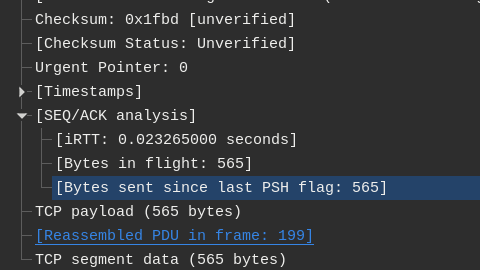
\includegraphics[width=0.7\linewidth]{upload_9dd059ac5700c7aa0441e5718c87d971.png}

For the first packet, the estimated RTT is equal to the calculated RTT
because we don't have any previous value.

\begin{enumerate}
\def\labelenumi{\arabic{enumi}.}
\setcounter{enumi}{7}
\item
  \begin{tabular}{|c|c|}
	  \hline
  Packet number & Length \\ \hline
  4 & 565 \\ \hline
  5 & 1460 \\ \hline
  7 & 1460 \\ \hline
  8 & 1460 \\ \hline
  10 & 1460 \\ \hline
  11 & 1460 \\ \hline
  \end{tabular}
\end{enumerate}

This length is taken in the Len TCP header.

\begin{enumerate}
\def\labelenumi{\arabic{enumi}.}
\setcounter{enumi}{8}
\item
  Window: 5840 (Window TCP header), It doesn't affect client because it
  always sends less than the window size.\\
  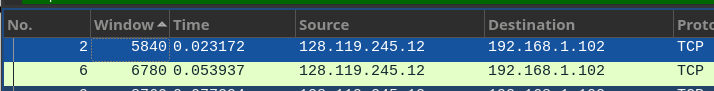
\includegraphics[width=0.7\linewidth]{upload_f2a87ad55988e55c582738446566f262.png}\\
  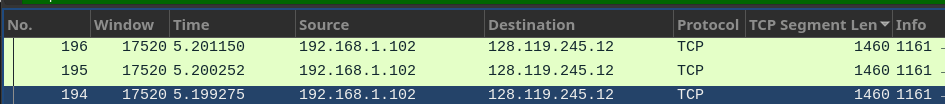
\includegraphics[width=0.7\linewidth]{upload_1d4a19c44f53f5db8f0cd7411ce33459.png}
\item
  There is no retransmitted segments. We checked RTT graph and for each
  packet there is an acknoledgement (no packet with infinite response
  time, continuous graph).\\
  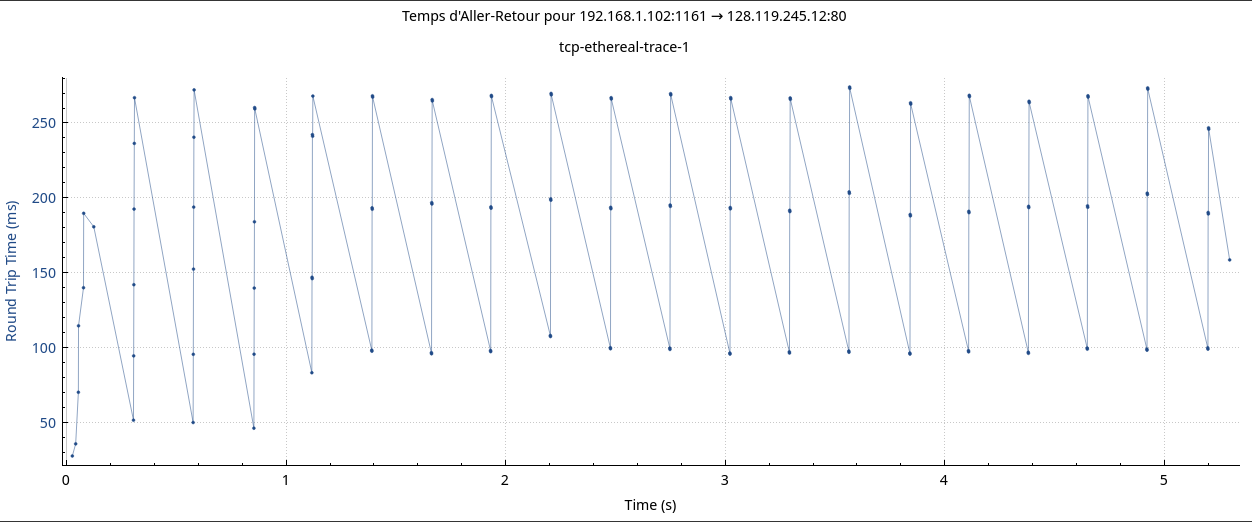
\includegraphics[width=0.7\linewidth]{upload_b63617d46a8846deeecfd63e107b094b.png}
\item
  The receiver acknowledge the last received packet in continuous data
  maybe the receiver ack more than one packet (for example packet 97
  acknoledge both 92 and 93 because the acknoledge number is 232201209
  and the previous one was 232198289 so it acknowledges 2920 bits of
  data more than the data sent in only one packet)
\item
  The total number of byte transferred is taken in the last transferred
  packet for the POST request, the Wireshark analyse show the number of
  bytes in the total of 122 TCP packets transferred for this request,
  164090 bytes. The total time is 5.297341000 seconds.
\end{enumerate}

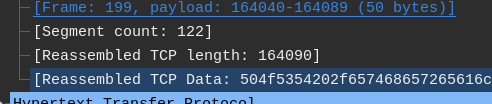
\includegraphics[width=0.7\linewidth]{upload_140917a895fff71033961f02b9f90110.png}\\
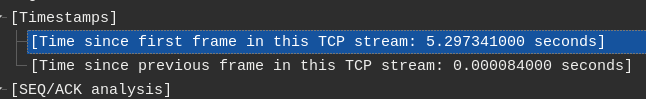
\includegraphics[width=0.7\linewidth]{upload_aaee14434fb3ed8d3e26b829b4d59ef6.png}

We use the following formula,
\(Throughput = (TransferredDataLength \times 8)/TimeSpendToSendPostRequest\).
The average throughput is between 200,000 to 250,000 bits/sec (247,807
bits/s). That is, 25,000 bytes/sec to 31,250 bytes/sec.

We saw here the principle of a TCP connection (connection oriented,
initialization of the connection, acknoledgement and sequence number)
with the different types of packets given the flags used in the TCP
headers.

We also experimented the calculated RTT and estimated RTT, the estimated
RTT is not really equal to the calculated RTT for example in this trace
where the connection is not very stable, the first value was very low
compared to the last ones and formula to estimate the RTT gives great
weight to the first values.

\chapter{TCP Congestion Control in action}

\begin{enumerate}
\def\labelenumi{\arabic{enumi}.}
\setcounter{enumi}{12}
\item
  The slow start phase is from the beginning (time 0) until the end of
  the transmission. There is no congestion avoidance because there is no
  retransmission, there is no decrease of the congestion window. The
  congestion window is bigger than 8192 that is the maximum number of
  unacknowledge bytes, we can find this by making the following table:
\end{enumerate}

\begin{longtable}{|c|c|c|c|}
	\hline
type & No & length & unacknowledged \\ \hline
\endhead
data & 4 & 565 & 565 \\ \hline
data & 5 & 1460 & 2025 \\ \hline
ack & 6 & 0 & 1460 \\ \hline
data & 7 & 1460 & 2920 \\ \hline
data & 8 & 1460 & 4380 \\ \hline
ack & 9 & 0 & 2920 \\ \hline
data & 10 & 1460 & 4380 \\ \hline
data & 11 & 1460 & 5840 \\ \hline
ack & 12 & 0 & 4380 \\ \hline
data & 13 & 1147 & 5527 \\ \hline
ack & 14 & 0 & 4067 \\ \hline
ack & 15 & 0 & 2607 \\ \hline
ack & 16 & 0 & 1147 \\ \hline
ack & 17 & 0 & 0 \\ \hline
data & 18 & 1460 & 1460 \\ \hline
data & 19 & 1460 & 2920 \\ \hline
data & 20 & 1460 & 4380 \\ \hline
data & 21 & 1460 & 5840 \\ \hline
data & 22 & 1460 & 7300 \\ \hline
data & 23 & 892 & 8192 \\ \hline
ack & 24 & 0 & 6732 \\ \hline
ack & 25 & 0 & 5272 \\ \hline
ack & 26 & 0 & 3812 \\ \hline
ack & 27 & 0 & 2352 \\ \hline
ack & 28 & 0 & 892 \\ \hline
ack & 29 & 0 & 0 \\ \hline
data & 30 & 1460 & 1460 \\ \hline
data & 31 & 1460 & 2920 \\ \hline
data & 32 & 1460 & 4380 \\ \hline
data & 33 & 1460 & 5840 \\ \hline
data & 34 & 1460 & 7300 \\ \hline
data & 35 & 892 & 8192 \\ \hline
ack & 36 & 0 & 6732 \\ \hline
ack & 37 & 0 & 5272 \\ \hline
ack & 38 & 0 & 3812 \\ \hline
ack & 39 & 0 & 2352 \\ \hline
ack & 40 & 0 & 892 \\ \hline
ack & 41 & 0 & 0 \\ \hline
data & 42 & 1460 & 1460 \\ \hline
data & 43 & 1460 & 2920 \\ \hline
data & 44 & 1460 & 4380 \\ \hline
data & 45 & 1460 & 5840 \\ \hline
data & 46 & 1460 & 7300 \\ \hline
data & 47 & 892 & 8192 \\ \hline
ack & 48 & 0 & 6732 \\ \hline
ack & 49 & 0 & 5272 \\ \hline
ack & 50 & 0 & 3812 \\ \hline
ack & 51 & 0 & 2352 \\ \hline
ack & 52 & 0 & 0 \\ \hline
data & 53 & 1460 & 1460 \\ \hline
data & 54 & 1460 & 2920 \\ \hline
data & 55 & 1460 & 4380 \\ \hline
data & 56 & 1460 & 5840 \\ \hline
data & 57 & 1460 & 7300 \\ \hline
data & 58 & 892 & 8192 \\ \hline
ack & 59 & 0 & 6732 \\ \hline
ack & 60 & 0 & 3812 \\ \hline
ack & 61 & 0 & 892 \\ \hline
ack & 62 & 0 & 0 \\ \hline
data & 63 & 1460 & 1460 \\ \hline
data & 64 & 1460 & 2920 \\ \hline
data & 65 & 1460 & 4380 \\ \hline
data & 66 & 1460 & 5840 \\ \hline
data & 67 & 1460 & 7300 \\ \hline
data & 68 & 892 & 8192 \\ \hline
ack & 69 & 0 & 5272 \\ \hline
ack & 70 & 0 & 2352 \\ \hline
ack & 71 & 0 & 0 \\ \hline
data & 72 & 1460 & 1460 \\ \hline
data & 73 & 1460 & 2920 \\ \hline
data & 74 & 1460 & 4380 \\ \hline
data & 75 & 1460 & 5840 \\ \hline
data & 76 & 1460 & 7300 \\ \hline
data & 77 & 892 & 8192 \\ \hline
ack & 78 & 0 & 5272 \\ \hline
ack & 79 & 0 & 2352 \\ \hline
ack & 80 & 0 & 0 \\ \hline
data & 81 & 1460 & 1460 \\ \hline
data & 82 & 1460 & 2920 \\ \hline
data & 83 & 1460 & 4380 \\ \hline
data & 84 & 1460 & 5840 \\ \hline
data & 85 & 1460 & 7300 \\ \hline
data & 86 & 892 & 8192 \\ \hline
ack & 87 & 0 & 5272 \\ \hline
ack & 88 & 0 & 2352 \\ \hline
ack & 89 & 0 & 0 \\ \hline
data & 90 & 1460 & 1460 \\ \hline
data & 91 & 1460 & 2920 \\ \hline
data & 92 & 1460 & 4380 \\ \hline
data & 93 & 1460 & 5840 \\ \hline
data & 94 & 1460 & 7300 \\ \hline
data & 95 & 892 & 8192 \\ \hline
ack & 96 & 0 & 5272 \\ \hline
ack & 97 & 0 & 2352 \\ \hline
ack & 98 & 0 & 0 \\ \hline
data & 99 & 1460 & 1460 \\ \hline
data & 100 & 1460 & 2920 \\ \hline
data & 101 & 1460 & 4380 \\ \hline
data & 102 & 1460 & 5840 \\ \hline
data & 103 & 1460 & 7300 \\ \hline
data & 104 & 892 & 8192 \\ \hline
ack & 105 & 0 & 5272 \\ \hline
ack & 106 & 0 & 2352 \\ \hline
ack & 107 & 0 & 0 \\ \hline
data & 108 & 1460 & 1460 \\ \hline
data & 109 & 1460 & 2920 \\ \hline
data & 110 & 1460 & 4380 \\ \hline
data & 111 & 1460 & 5840 \\ \hline
data & 112 & 1460 & 7300 \\ \hline
data & 113 & 892 & 8192 \\ \hline
ack & 114 & 0 & 5272 \\ \hline
ack & 115 & 0 & 2352 \\ \hline
ack & 116 & 0 & 0 \\ \hline
data & 117 & 1460 & 1460 \\ \hline
data & 118 & 1460 & 2920 \\ \hline
data & 119 & 1460 & 4380 \\ \hline
data & 120 & 1460 & 5840 \\ \hline
data & 121 & 1460 & 7300 \\ \hline
data & 122 & 892 & 8192 \\ \hline
ack & 123 & 0 & 5272 \\ \hline
ack & 124 & 0 & 2352 \\ \hline
ack & 125 & 0 & 0 \\ \hline
data & 126 & 1460 & 1460 \\ \hline
data & 127 & 1460 & 2920 \\ \hline
data & 128 & 1460 & 4380 \\ \hline
data & 129 & 1460 & 5840 \\ \hline
data & 130 & 1460 & 7300 \\ \hline
data & 131 & 892 & 8192 \\ \hline
ack & 132 & 0 & 5272 \\ \hline
ack & 133 & 0 & 2352 \\ \hline
ack & 134 & 0 & 0 \\ \hline
data & 135 & 1460 & 1460 \\ \hline
data & 136 & 1460 & 2920 \\ \hline
data & 137 & 1460 & 4380 \\ \hline
data & 138 & 1460 & 5840 \\ \hline
data & 139 & 1460 & 7300 \\ \hline
data & 140 & 892 & 8192 \\ \hline
ack & 141 & 0 & 5272 \\ \hline
ack & 142 & 0 & 2352 \\ \hline
ack & 143 & 0 & 0 \\ \hline
data & 144 & 1460 & 1460 \\ \hline
data & 145 & 1460 & 2920 \\ \hline
data & 146 & 1460 & 4380 \\ \hline
data & 147 & 1460 & 5840 \\ \hline
data & 148 & 1460 & 7300 \\ \hline
data & 149 & 892 & 8192 \\ \hline
ack & 150 & 0 & 5272 \\ \hline
ack & 151 & 0 & 2352 \\ \hline
ack & 152 & 0 & 0 \\ \hline
data & 153 & 1460 & 1460 \\ \hline
data & 154 & 1460 & 2920 \\ \hline
data & 155 & 1460 & 4380 \\ \hline
data & 156 & 1460 & 5840 \\ \hline
data & 157 & 1460 & 7300 \\ \hline
data & 158 & 892 & 8192 \\ \hline
ack & 159 & 0 & 5272 \\ \hline
ack & 160 & 0 & 2352 \\ \hline
ack & 161 & 0 & 0 \\ \hline
data & 162 & 1460 & 1460 \\ \hline
data & 163 & 1460 & 2920 \\ \hline
data & 164 & 1460 & 4380 \\ \hline
data & 165 & 1460 & 5840 \\ \hline
data & 166 & 1460 & 7300 \\ \hline
data & 167 & 892 & 8192 \\ \hline
ack & 168 & 0 & 5272 \\ \hline
ack & 169 & 0 & 2352 \\ \hline
ack & 170 & 0 & 0 \\ \hline
data & 171 & 1460 & 1460 \\ \hline
data & 172 & 1460 & 2920 \\ \hline
data & 173 & 1460 & 4380 \\ \hline
data & 174 & 1460 & 5840 \\ \hline
data & 175 & 1460 & 7300 \\ \hline
data & 176 & 892 & 8192 \\ \hline
ack & 177 & 0 & 5272 \\ \hline
ack & 178 & 0 & 2352 \\ \hline
ack & 179 & 0 & 0 \\ \hline
data & 180 & 1460 & 1460 \\ \hline
data & 181 & 1460 & 2920 \\ \hline
data & 182 & 1460 & 4380 \\ \hline
data & 183 & 1460 & 5840 \\ \hline
data & 184 & 1460 & 7300 \\ \hline
data & 185 & 892 & 8192 \\ \hline
ack & 186 & 0 & 5272 \\ \hline
ack & 190 & 0 & 2352 \\ \hline
ack & 191 & 0 & 0 \\ \hline
data & 192 & 1460 & 1460 \\ \hline
data & 193 & 1460 & 2920 \\ \hline
data & 194 & 1460 & 4380 \\ \hline
data & 195 & 1460 & 5840 \\ \hline
data & 196 & 1460 & 7300 \\ \hline
data & 197 & 272 & 7572 \\ \hline
ack & 198 & 0 & 4652 \\ \hline
data & 199 & 50 & 4702 \\ \hline
ack & 200 & 0 & 1782 \\ \hline
ack & 201 & 0 & 50 \\ \hline
ack & 202 & 0 & 0 \\ \hline
\end{longtable}

Here the congestion window is never increased after 8192, so we remain
in the slow start phase, we never have congestion avoidance or AIMD.

\begin{enumerate}
\def\labelenumi{\arabic{enumi}.}
\setcounter{enumi}{13}
\item
  LastByteSent -- LastByteAcked \textless= min\{cwnd, rwnd\}. If we send
  more data than one of two windows (congestion and receiver), there is
  a risk of data losses because the network or the receiver can't handle
  this amount of data. The effective window is the minimum between cwnd
  and rwnd. The effective window seems to be the congestion window
  because we are always far from the receiver window.
\item
  We can't have the real value of the congestion window from the dump,
  because this is calculated by the sender and not part of the TCP
  headers but we know that the number of sent data is always smaller
  than the congestion window. The congestion window could be 8192 for
  example but we have less than 8192 bytes of data to send so we can't
  estimate the congestion window, we can only have a upper bound.
\end{enumerate}

\chapter{A Short Study of TCP fairness}

\[
Average Troughput = (1.22 \times MSS) / (RTT \times \sqrt{L})
\]

\begin{enumerate}
\def\labelenumi{\arabic{enumi}.}
\setcounter{enumi}{15}
\item
  Throughput (bits / sec) = ((Total bytes) * 8) (bits) / Duration (sec)\\
      \begin{tabular}{|l|l|l|l|l|}
    \hline
        Connection & Total bytes & Duration & RTT & throughput \\ \hline
        1 & 165095720 & 521 & 12 & 2535059.0403071 \\ \hline
        2 & 165842766 & 521 & 12 & 2546529.99616123 \\ \hline
        3 & 165458792 & 514 & 12 & 2575234.11673152 \\ \hline
        4 & 163235772 & 512 & 12 & 2550558.9375 \\ \hline
    \end{tabular}
\end{enumerate}

Each TCP connection has a throughput of approximatly 2.5 Mb/s Total
Bandwidth = 10207382.0906998 = 10Mb/s

The TCP connection throughput is almost equal between each client in
this case, so fair.

\begin{enumerate}
\def\labelenumi{\arabic{enumi}.}
\setcounter{enumi}{16}
\item
  Throughput (bits / sec) = ((Total bytes) * 8) (bits) / Duration (sec)\\
      \begin{tabular}{|l|l|l|l|l|}
    \hline
        Connection & Total bytes & Duration & RTT & throughput \\ \hline
        1 & 261319130 & 90 & 13 & 23228367.11 \\ \hline
        2 & 175995832 & 90 & 35 & 15644073.96 \\ \hline
        3 & 151894552 & 90 & 68 & 13501737.96 \\ \hline
        4 & 140388568 & 90 & 73 & 12478983.82 \\ \hline
        5 & 108610702 & 90 & 49 & 9654284.622 \\ \hline
        6 & 70644690 & 90 & 33 & 6279528 \\ \hline
        7 & 65744938 & 90 & 135 & 5843994.489 \\ \hline
        8 & 43212876 & 90 & 326 & 3841144.533 \\ \hline
        9 & 39222524 & 90 & 322 & 3486446.578 \\ \hline
    \end{tabular}
\end{enumerate}

Total Bandwidth = 93958561.07 = 94Mb/s The range of each TCP connection
throughput is 3Mb/s \textasciitilde{} 23Mb/s.

The TCP connection throughput is various between each client in this
case, so not so fair. For example connection 2 and 6 have almost the
same RTT but we have a very different throughput. But 3 and 4 are almost
fair, the difference comes from the bigger RTT in the connection 4.

\begin{enumerate}
\def\labelenumi{\arabic{enumi}.}
\setcounter{enumi}{17}
\item
  Throughput (bits / sec) = ((Total bytes) * 8) (bits) / Duration (sec)\\
      \begin{tabular}{|l|l|l|l|l|}
    \hline
        Connection & Total bytes & Duration & RTT & throughput \\ \hline
        1 & 108851134 & 58 & 40 & 9675656.356 \\ \hline
        2 & 90435681 & 58 & 36 & 8038727.2 \\ \hline
        3 & 57971584 & 53 & 100 & 5153029.689 \\ \hline
        4 & 32000012 & 29 & 68 & 2844445.511 \\ \hline
        5 & 32557334 & 35 & 31 & 2893985.244 \\ \hline
        6 & 27199361 & 31 & 32 & 2417720.978 \\ \hline
        7 & 26329578 & 31 & 122 & 2340406.933 \\ \hline
        8 & 38834490 & 56 & 146 & 3451954.667 \\ \hline
        9 & 23571761 & 35 & 74 & 2095267.644 \\ \hline
        10 & 36252962 & 55 & 66 & 3222485.511 \\ \hline
    \end{tabular}
\end{enumerate}

The TCP connection throughput is various between each client but not
much various as question 17 case.

With bittorrent we have multiple connections to transfer one file, so
the total bandwidth for the file is greater than the total bandwith with
an HTTP connection for example.
\end{document}
